\subsection{Type of Variable}
\label{sec:history}
In Rust, there are three variable types: owner, reference, and slice (only for sequence of values). 
A developer is sometimes forced to use specific variable types. For example, some of methods are only implemented to specific variable types.
However, one can select any variable types for operation in most case.

These variables have different memory representation shown in Figure~\ref{fig:own_ref_slice}.
The owner has a pointer pointing to the memory address of sequence values, length of the values, and capacity allocated to store additional values. 
Reference and Slice are variables borrowing value owned by other variable. The reference is a pointer that points to the owner. 
The slice is a pointer that points to memory address of sequence values. It has value such as length of sequence values stored in the memory. 
Since they have different memory representation, an assumption is that it takes different time to access to the contents of the memory among these pointer types.
We examine this by constructing complex objects whose fields are these variable types. The details are explained in section 3.2.

\begin{figure}[htb]
    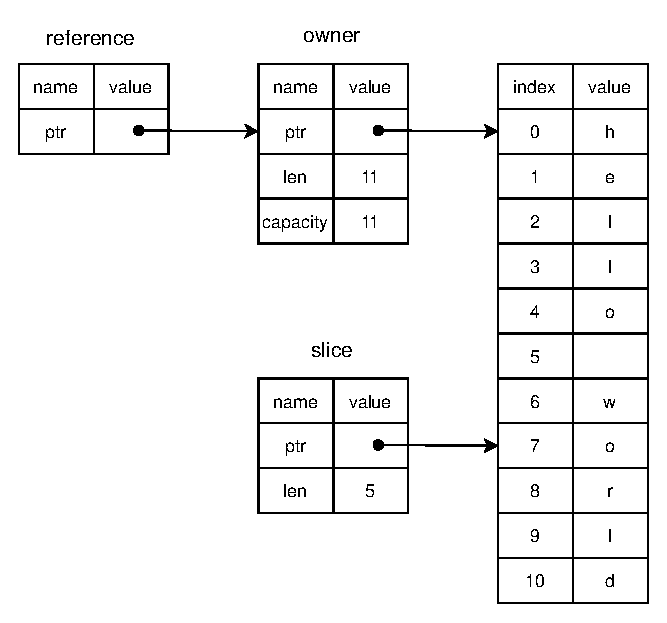
\includegraphics[width=10cm]{own_ref_slice.eps}
    \caption{Memory Representation of Owner, Reference, and Slice Type}
    \label{fig:own_ref_slice}
\end{figure}

\subsection{Reference Count}
\label{sec:history}
Reference is useful to avoid movement of ownership. However, one needs to track its lifetime and explicitly includes it in code, 
because Rust compiler cannot infer it. This can be another encumbrance. We can instead acquire multiple owners to single value by using Reference Counting (Rc). 
By leveraging Rc, a value can be shared like what borrowing plays the role in Rust programming. 

The difference is that Rc checks number of owner pointing to the actual data and makes sure the data is not deleted 
until all the owners are dereferenced. Using Rc is sometimes preferable approach for developers especially when lifetime planning is extremely difficult.
However, the possible problem regarding to Rc is the cost for tracking the number of references. 
Having this assumption, an experiment is conducted to examine difference of runtime performance of dropping reference and Rc. 
This is explained in section 3.2.

\subsection{Multithreading}
\label{sec:history}
In Rust programming, writing concurrent code is relatively easy. The care Rust takes with reference, mutability, and lifetimes is valuable enough in single-threaded programs, 
but it also is in concurrent programming. Rust has tools to write concurrent code, such as threads, locks, atomic reference. 
Therefore, one can implement various concurrent codes for the same purpose with different memory management strategies. 
The most ubiquitous tool used in Rust concurrent code is Atomic Reference Counting (Arc). 

Arc is a simple interface that allows threads to share data. Arc allows multiple variable to have ownerships of a particular value similarly to Rc, 
but also supports atomic feature enabling the ownerships exist in different threads. 
In many situation where developer write a multithreading code, the deletion of Arc happens significant amount of times. 
Similarly to Rc, our assumption is that deletion of Arc has also overhead when we compare to normal reference. 
To assess runtime performances of algorithm with Arc vs normal reference, we implement merge-sort algorithm in two different ways. 

\subsection{Algorithm in Big Data}
\label{sec:history}
Finally, we implement some of algorithm common in Big Data processing: Tree-aggregate and K-Nearest-Neighbors (KNN). 

Tree-aggregate is a communication patten heavily used for Machine Learning algorithm in Spark (MLlib). 
In the traditional aggregation function in Spark, results of aggregation in all executor clusters are sent to the driver. 
That is why this operation suffers from the CPU cost in merging partial results and the network bandwidth limit.
Tree-aggregate is a communication pattern which overcomes these problems by breaking aggregate operation in multi-level represented like tree structure.

KNN is a traditional Machine Learning algorithm which classify targets into categories. 
Through experiments with these algorithm, we aim to find algorithm with understandability and efficiency. 
\clearpage
